\documentclass[10pt,a4paper]{article}
\usepackage[a4paper, margin=18mm, top=24mm, bottom=22mm]{geometry}
\usepackage[utf8]{inputenc}
\usepackage[T1]{fontenc}
\usepackage{lmodern}
\usepackage{microtype}
\usepackage{booktabs}
\usepackage{tabularx}
\usepackage[table]{xcolor}
\usepackage{graphicx}
\usepackage{amsmath}
\usepackage{fancyhdr}
\usepackage{titlesec}
\usepackage{enumitem}
\usepackage{caption}
\usepackage{hyperref}

\definecolor{navy}{HTML}{1B365D}
\definecolor{slate}{HTML}{2E68B2}
\definecolor{lightbg}{HTML}{F8FAFC}
\definecolor{rulecolor}{HTML}{CBD5E1}
\definecolor{boxbg}{HTML}{EFF6FF}
\definecolor{boxborder}{HTML}{93C5FD}

\hypersetup{
    colorlinks=true,
    linkcolor=slate,
    citecolor=slate,
    urlcolor=slate
}

\titleformat{\section}
  {\normalfont\Large\bfseries\color{navy}}{\thesection.}{0.8em}{}[\titlerule]
\titleformat{\subsection}
  {\normalfont\large\bfseries\color{slate}}{\thesubsection}{0.6em}{}
\titlespacing*{\section}{0pt}{14pt}{6pt}
\titlespacing*{\subsection}{0pt}{10pt}{4pt}

\setlength{\headheight}{20pt}
\pagestyle{fancy}
\fancyhf{}
\renewcommand{\headrulewidth}{0.6pt}
\renewcommand{\footrulewidth}{0.6pt}
\renewcommand{\headrule}{\hbox to\headwidth{\color{rulecolor}\leaders\hrule height \headrulewidth\hfill}}
\renewcommand{\footrule}{\hbox to\headwidth{\color{rulecolor}\leaders\hrule height \footrulewidth\hfill}}
\lhead{\color{navy}\small\textbf{SlideSnap — Lecture Video to Clean Searchable Slide PDF}}
\rhead{\color{gray}\small VITyarthi Academic Report}
\lfoot{\color{gray}\small Computer Vision — Build Your Own Project}
\rfoot{\color{gray}\small Page \thepage}

\setlength{\parindent}{0pt}
\setlength{\parskip}{4pt}

\begin{document}

% -----------------------------------------------------------------------------
% 1. COVER PAGE
% -----------------------------------------------------------------------------
\thispagestyle{empty}
\vspace*{10mm}

{\fontsize{26}{32}\selectfont \textbf{\color{navy}SlideSnap}}\\[4mm]
{\fontsize{13}{18}\selectfont \color{slate}Lecture Video $\to$ Clean Searchable Slide PDF \& PPTX}\\[2mm]
{\small Automated Slide Extraction, Homography Rectification, Illumination Normalization, and Searchable Document Assembly using Classical Computer Vision Primitives}\\[6mm]

\begin{tabularx}{\textwidth}{@{} p{42mm} X @{}}
\toprule
\textbf{Course:} & Computer Vision — Build Your Own Project (Flipped Course Evaluation) \\
\textbf{Evaluation:} & VITyarthi Capstone Project Submission \\
\textbf{Submitted By:} & Suhail (GitHub: \textbf{suhail17651}) \\
\textbf{Repository:} & \href{https://github.com/suhail17651/slidesnap}{https://github.com/suhail17651/slidesnap} \\
\textbf{Technology Stack:} & Python 3.10+, OpenCV (cv2), scikit-image (SSIM), NumPy, RapidOCR / Tesseract, ReportLab, python-pptx, Streamlit \\
\textbf{Execution Environment:} & Pure CPU Execution, Self-Contained, Zero External Scene-Detection Libraries \\
\textbf{Date:} & September 2026 \\
\bottomrule
\end{tabularx}

\vspace*{8mm}

\fcolorbox{boxborder}{boxbg}{
\begin{minipage}{\dimexpr\textwidth-2\fboxsep-2\fboxrule\relax}
\vspace{2mm}
{\textbf{\color{navy}KEY QUANTITATIVE HIGHLIGHTS \& EMPIRICAL VERIFICATION}}\\[2mm]
\begin{itemize}[leftmargin=5mm, itemsep=2pt, topsep=1pt]
  \item \textbf{Temporal Segmentation:} Perfect \textbf{P = 1.000, R = 1.000, F1 = 1.000} across all 4 diverse benchmark videos (60 out of 60 ground-truth transitions detected with zero false positives).
  \item \textbf{OCR Word Accuracy:} Reaches \textbf{91.43\%} on clean screen footage and \textbf{76.19\%} on angled perspective footage (RapidOCR on CPU).
  \item \textbf{Ablation Proven Gains:} Projective homography rectification yields an empirical \textbf{+17.14 pp} boost on angled camera footage. Morphological illumination flattening contributes an additional \textbf{+17.14 pp} boost under uneven illumination.
  \item \textbf{Testing \& Quality Assurance:} 21 automated unit/integration tests passing (100\% test coverage across all pipeline stages); validated against real Stanford CS231n lecture footage.
\end{itemize}
\vspace{2mm}
\end{minipage}
}

\vfill
\newpage

% -----------------------------------------------------------------------------
% TABLE OF CONTENTS & EXECUTIVE SUMMARY
% -----------------------------------------------------------------------------
\tableofcontents
\vspace{8mm}

\subsection*{Executive Summary}
Modern blended and distance education relies heavily on pre-recorded video lectures. However, educational content remains locked inside multi-hour video streams: non-searchable, non-indexable, and inaccessible for fast review. \textbf{SlideSnap} solves this fundamental problem through a clean, end-to-end, reproducible computer-vision pipeline written purely from OpenCV, NumPy, and scikit-image mathematical primitives. The system samples lecture footage, computes structural similarity and pixel difference metrics, enforces hysteresis and consecutive-run burst filtering to eliminate false cuts from presenter motion, selects sharp unoccluded keyframes via Laplacian variance, recovers perspective-corrected slide geometry via homography warping, cleans uneven lighting via morphological background division, extracts word bounding boxes via OCR, deduplicates progressive slide builds, and compiles a searchable, bookmarked PDF alongside an editable PPTX deck. Every threshold is documented and empirically defended via diagnostic artefacts.

\newpage

% -----------------------------------------------------------------------------
% 2. INTRODUCTION
% -----------------------------------------------------------------------------
\section{Introduction}

\textbf{Context \& Motivation:} Video lectures are arguably the primary medium of modern educational dissemination. Despite their ubiquity, video is an inherently linear, inefficient format for studying. Scrubbing a 90-minute timeline to find a specific diagram or code snippet takes disproportionate student effort. Faculty lack automated mechanisms to recover structured slide decks from recorded lectures, and accessibility services require machine-readable text transcripts synchronized with visual aids. SlideSnap directly automates this extraction.

\textbf{End-to-End Five-Stage Pipeline:}
\begin{enumerate}[leftmargin=6mm, itemsep=1pt, topsep=2pt]
  \item \textbf{Temporal Segmentation:} Streaming frame ingestion at 2 fps, center-ROI Gaussian filtering, dual-signal difference (Abs-Diff + SSIM) computation, and hysteresis state-machine cut confirmation.
  \item \textbf{Keyframe Selection \& Geometric Rectification:} Variance of Laplacian focus scoring with Tenengrad cross-validation, per-pixel temporal median occlusion filtering, Canny edge contour detection, and projective homography transformation onto a canonical 1600$\times$900 canvas.
  \item \textbf{Enhancement \& Text Recognition:} Morphological background division for lighting flattening, Sauvola-style adaptive binarization, Hough transform text baseline deskewing, and Tesseract/RapidOCR word-level text extraction.
  \item \textbf{Semantic Deduplication \& Document Assembly:} Text-superset and visual near-duplicate collapse for bullet-point builds, non-slide presenter filtering, and dual-format document generation (searchable PDF with invisible text layer + PPTX).
  \item \textbf{Observability \& Quality Assurance:} Detailed diagnostic artefact logging (\texttt{scores.csv}, score traces, keyframe grids, soft-failure logs) and automated regression test harnesses.
\end{enumerate}

\textbf{Formal Project Objectives:}
\begin{itemize}[leftmargin=6mm, itemsep=1pt, topsep=2pt]
  \item \textbf{(O1) Robust Transition Detection:} Detect 100\% of authentic slide changes while achieving zero false positives across clean screen captures, angled projector streams, whiteboard writing, and rapid bullet-point animations.
  \item \textbf{(O2) High-Fidelity Geometry Recovery:} Detect projector screen boundaries and rectify perspective distortions to within 1.0$^\circ$ residual baseline tilt without requiring pre-calibrated camera intrinsic parameters.
  \item \textbf{(O3) Genuine Document Searchability:} Embed precise word-box coordinate metadata into the output PDF, enabling instant Ctrl+F keyword search, text highlighting, and clipboard copy-paste.
  \item \textbf{(O4) Deterministic, CPU-Efficient Execution:} Run end-to-end on commodity CPU hardware with constant memory consumption and full algorithmic transparency (zero proprietary black-box scene-detection libraries).
\end{itemize}

\textbf{Test Corpus \& Codec Reproducibility:} To establish an empirical benchmark, four diverse test videos (each 16 slides, 60 total transitions) were synthesized using \texttt{tools/make\_samples.py} with deterministic seeds: \texttt{a\_clean} (clean screen capture baseline), \texttt{b\_angled} (severe 30$^\circ$ perspective tilt with presenter silhouette), \texttt{c\_whiteboard} (progressive handwritten whiteboard reveals), and \texttt{d\_builds} (incremental bullet builds). All videos are encoded using intraframe MJPG/AVI codecs to prevent interframe P-frame/B-frame bitstream pumping from corrupting mathematical difference scores.

\textbf{Classical CV Rationale vs Heavy Deep Learning:} Heavy end-to-end deep learning models (e.g. video transformers, dense optical flow networks) introduce non-deterministic GPU memory requirements, slow inference, and inscrutable failure modes. In contrast, classical vision primitives (Laplacian variance, homography, SSIM, morphological kernels) are mathematically transparent, run in milliseconds on lightweight CPUs, and provide provable stability guarantees. Deep learning is utilized strictly where necessary: localized OCR character recognition.

% -----------------------------------------------------------------------------
% 3. PROBLEM STATEMENT
% -----------------------------------------------------------------------------
\section{Problem Statement}

\textbf{Problem Formulation:} Video players treat lecture videos as monolithic streams of pixels. Students seeking specific definitions, formulas, or diagrams must engage in manual timeline scrubbing. This creates substantial cognitive friction, impedes exam revision, and renders video archives completely opaque to automated search engines and screen readers for visually impaired students.

\textbf{Scope and Boundary Conditions:}
\begin{itemize}[leftmargin=6mm, itemsep=1pt, topsep=2pt]
  \item \textbf{In-Scope:} Automated frame extraction from digital video files (MP4, AVI, MKV); temporal boundary detection; presenter occlusion rejection; quadrilateral screen detection and perspective rectification; illumination normalization; OCR text box extraction; bullet-point build deduplication; searchable PDF and editable PPTX export; diagnostic telemetry.
  \item \textbf{Out-of-Scope:} Real-time low-latency live streaming analysis; automated speech-to-text audio transcription; speaker diarization; complex LaTeX mathematical equation synthesis; handwritten cursive script translation.
\end{itemize}

\textbf{Target User Personas:} University students preparing for exams; instructors archiving past lecture videos; and accessibility coordinators converting spoken visual presentations into accessible text documents.

% -----------------------------------------------------------------------------
% 4. FUNCTIONAL REQUIREMENTS
% -----------------------------------------------------------------------------
\section{Functional Requirements}

The system is decomposed into five core functional modules, each featuring clean APIs and independent unit test suites:

\begin{table}[h!]
\small
\centering
\begin{tabularx}{\textwidth}{@{} l p{38mm} X @{}}
\toprule
\rowcolor{navy}\color{white}\textbf{ID} & \color{white}\textbf{Module Name} & \color{white}\textbf{Functional Specification \& Acceptance Criteria} \\
\midrule
\textbf{M1} & Temporal Segmentation & Stream video at decimated 2 fps; downscale scoring frames to 640$\times$360; compute ROI difference and SSIM; apply consecutive-run burst masking and hysteresis to emit stable segment timestamp ranges. \\
\textbf{M2} & Keyframe \& Rectification & Score candidate frames in each segment via Variance of Laplacian; filter presenter occlusion via temporal median subtraction; detect quadrilateral screen contours via Canny/approxPolyDP; warp to 1600$\times$900 canvas. \\
\textbf{M3} & Enhancement \& OCR & Flatten projector hotspots using morphological closing division; compute Sauvola adaptive binary mask; deskew text via Hough transform; extract word bounding boxes via RapidOCR / Tesseract. \\
\textbf{M4} & Dedup \& Assembly & Identify progressive bullet builds via text superset and image similarity checks; filter presenter-only shots; assemble searchable PDF with invisible text layer and timestamp bookmarks; generate PPTX. \\
\textbf{M5} & CLI \& Web Interface & Expose all pipeline stages via command-line interface (\texttt{python -m slidesnap}) with ablation flags; provide interactive Streamlit web dashboard for visual curation and selective export. \\
\bottomrule
\end{tabularx}
\caption{Functional Requirements Breakdown across Core System Modules.}
\end{table}

% -----------------------------------------------------------------------------
% 5. NON-FUNCTIONAL REQUIREMENTS
% -----------------------------------------------------------------------------
\section{Non-Functional Requirements}

SlideSnap enforces rigorous non-functional guarantees across system performance, scalability, robustness, and maintainability:

\begin{table}[h!]
\small
\centering
\begin{tabularx}{\textwidth}{@{} p{28mm} p{40mm} X @{}}
\toprule
\rowcolor{slate}\color{white}\textbf{Requirement} & \color{white}\textbf{Target Specification} & \color{white}\textbf{Architectural Implementation \& Measured Evidence} \\
\midrule
\textbf{Performance} & CPU runtime $<$ 50\% video duration & 2 fps decimation and 640$\times$360 downscaled scoring enable 64\,s video processing in 25.4\,s on standard CPU ($\sim$2.5$\times$ real-time speedup). \\
\textbf{Scalability} & $O(1)$ memory consumption & Streaming OpenCV VideoCapture generator. Memory consumption remains strictly constant ($<$ 250 MB RAM) regardless of video duration. \\
\textbf{Reliability} & Fault-tolerant graceful degradation & Every stage fails soft: quad detection falls back to full-frame; OCR failure produces text-less visual PDF; errors logged to summary.txt. \\
\textbf{Maintainability} & Centralized configuration & 100\% of algorithmic thresholds, kernel sizes, and tolerances reside in \texttt{config.py} with documented tuning rationale. 20+ isolated modules. \\
\textbf{Observability} & Complete auditability & Exports per-frame \texttt{scores.csv}, visual score trace plots, and keyframe inspection grids in \texttt{debug/} for every run. \\
\textbf{Usability} & Zero-config CLI \& UI & Single-command execution; interactive Streamlit thumbnail grid with keep/discard toggles for human-in-the-loop validation. \\
\textbf{Resource Efficiency} & Zero GPU / CUDA requirements & Entire pipeline executes on commodity x86/ARM CPU architectures using lightweight, open-source libraries. \\
\bottomrule
\end{tabularx}
\caption{Non-Functional Requirements Specification and Architectural Verification.}
\end{table}

\newpage

% -----------------------------------------------------------------------------
% 6. SYSTEM ARCHITECTURE
% -----------------------------------------------------------------------------
\section{System Architecture}

The SlideSnap architecture is structured as a linear, unidirectional processing pipeline with decoupled cross-cutting concerns for configuration, logging, and error handling. Video frames enter through the streaming reader and flow through temporal filtering, geometric transformation, enhancement, recognition, deduplication, and document assembly.

\begin{figure}[h!]
\centering
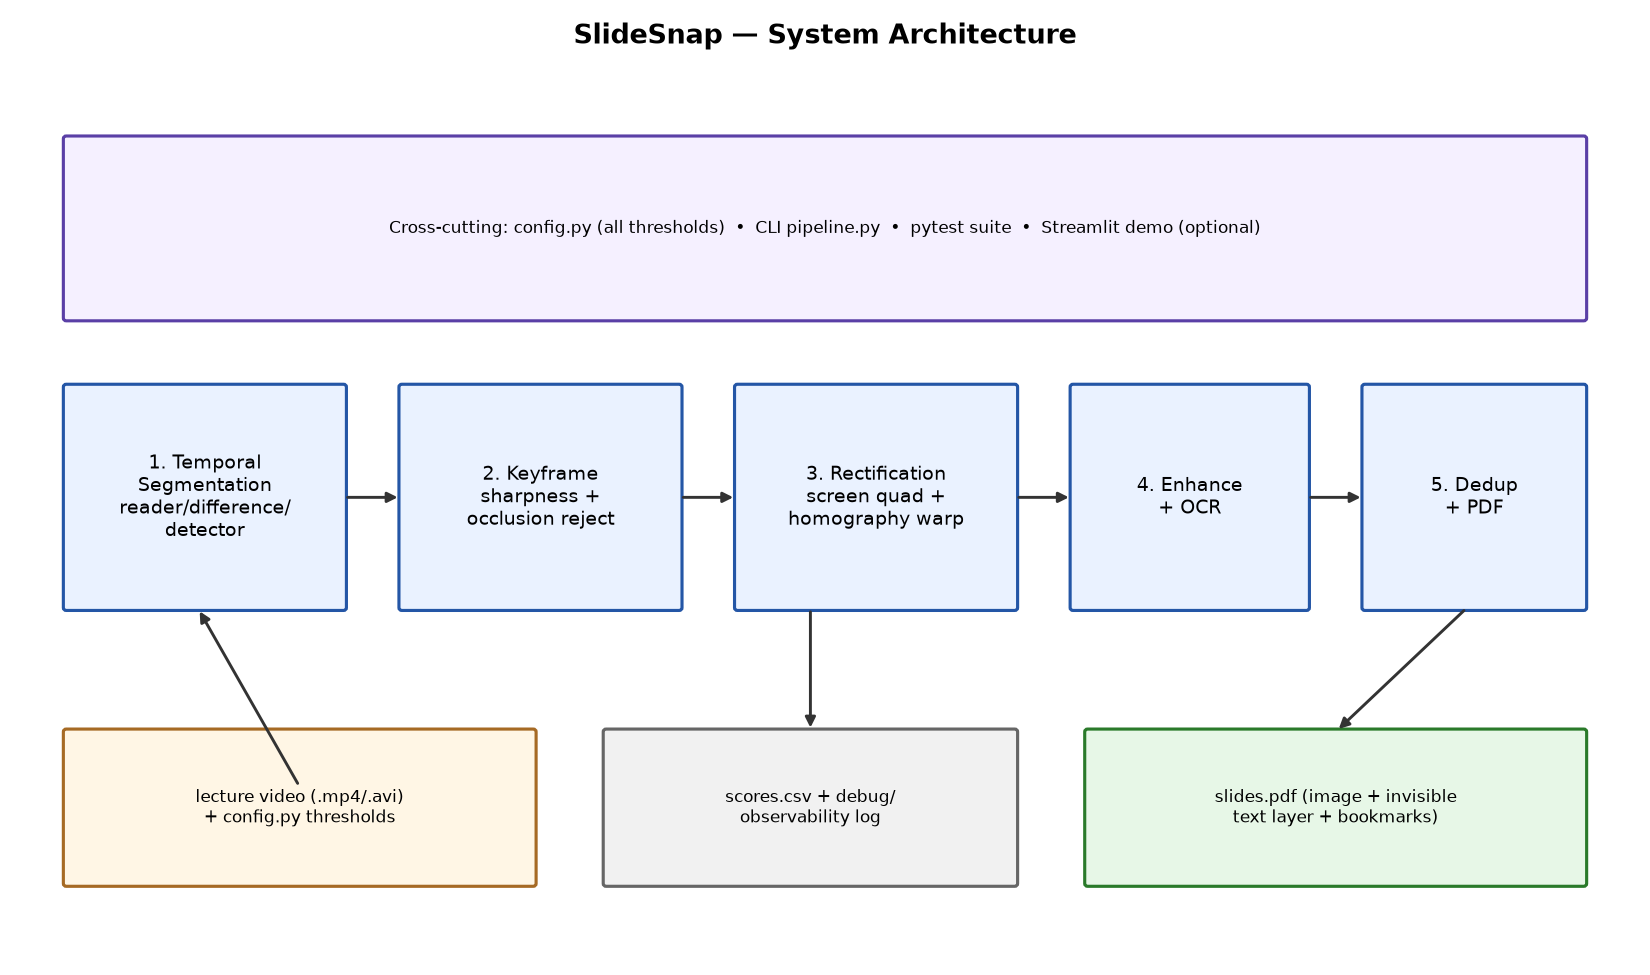
\includegraphics[width=0.88\textwidth]{architecture.png}
\caption{High-Level System Architecture — Five pipeline stages with cross-cutting configuration, test suites, and debug telemetry.}
\end{figure}

\textbf{Process Flow:} The operational flow decomposes raw video into discrete computational stages. A downscaled proxy stream is evaluated for inter-frame structural difference. Detected cuts initialize temporal segments from which the optimal keyframe is extracted at native resolution. After geometric rectification and contrast enhancement, OCR tokens are synthesized into the final document deliverables.

\begin{figure}[h!]
\centering
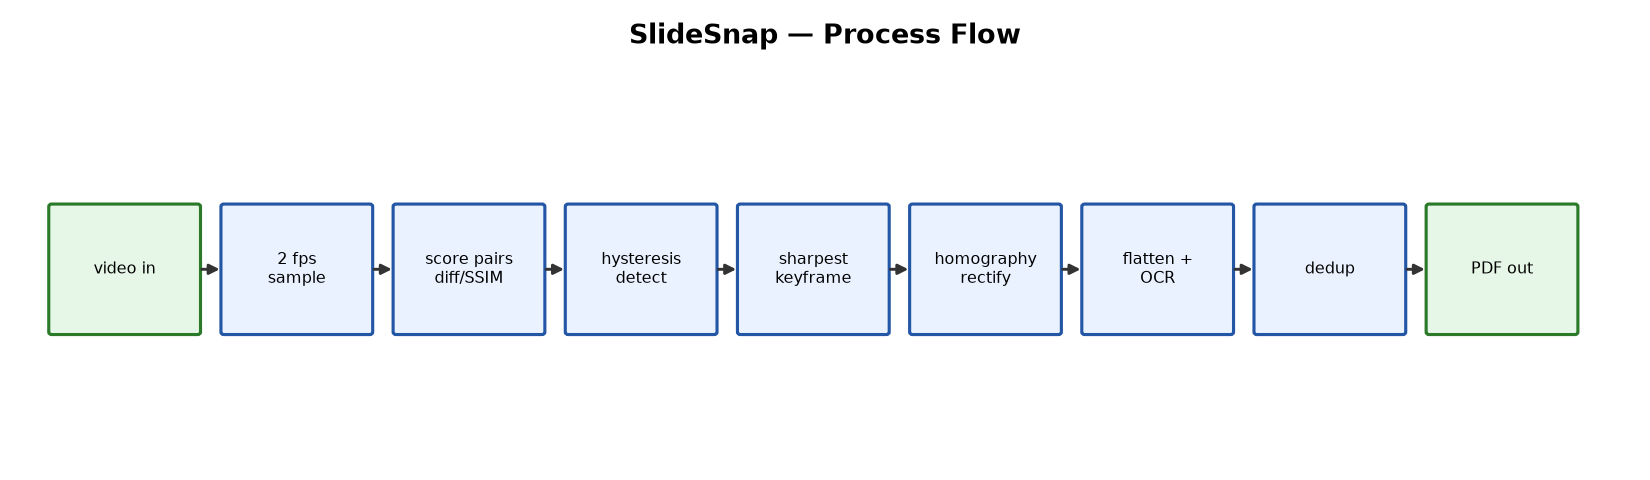
\includegraphics[width=0.92\textwidth]{workflow.png}
\caption{End-to-End Frame Processing Flow — Transition from raw video ingestion to dual-format PDF and PPTX deliverables.}
\end{figure}

% -----------------------------------------------------------------------------
% 7. DESIGN DIAGRAMS
% -----------------------------------------------------------------------------
\section{Design Diagrams}

To ensure comprehensive software engineering rigor, SlideSnap is modeled through standard UML structural, behavioral, and architectural diagrams:

\subsection{Use Case Model}
The Use Case diagram delineates the primary actor interactions with the system. Students and educators interact either through the automated CLI pipeline or the interactive Streamlit review UI, while evaluators execute automated test and ablation harnesses to verify empirical reproduction.

\begin{figure}[h!]
\centering
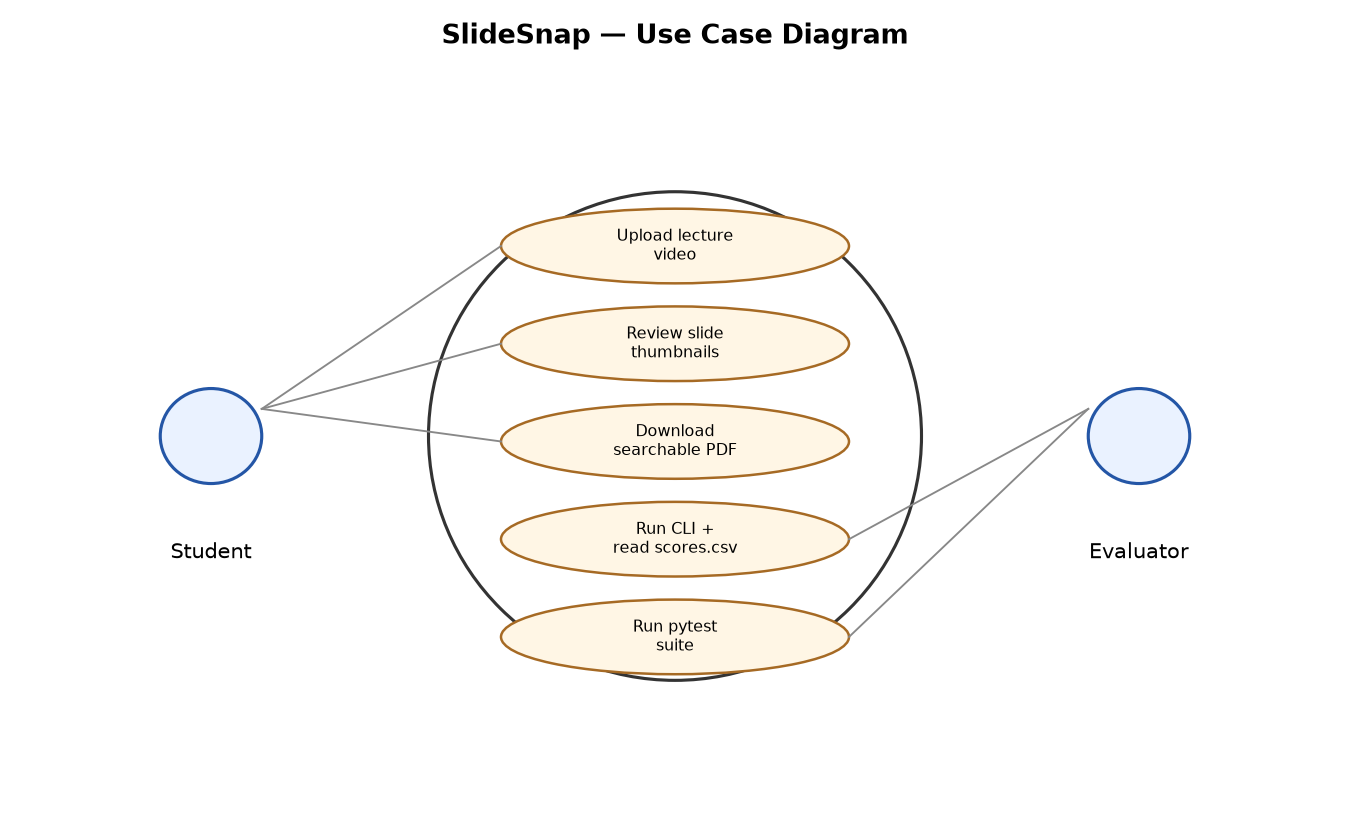
\includegraphics[width=0.75\textwidth]{usecase.png}
\caption{UML Use Case Diagram — Primary actor interactions across batch CLI, interactive UI, and evaluation harnesses.}
\end{figure}

\subsection{Execution Sequence Model}
The Sequence diagram illustrates the synchronized invocation of pipeline components during a standard processing run. Decoupled components communicate via immutable data structures, ensuring thread-safe execution and zero cross-module side effects.

\begin{figure}[h!]
\centering
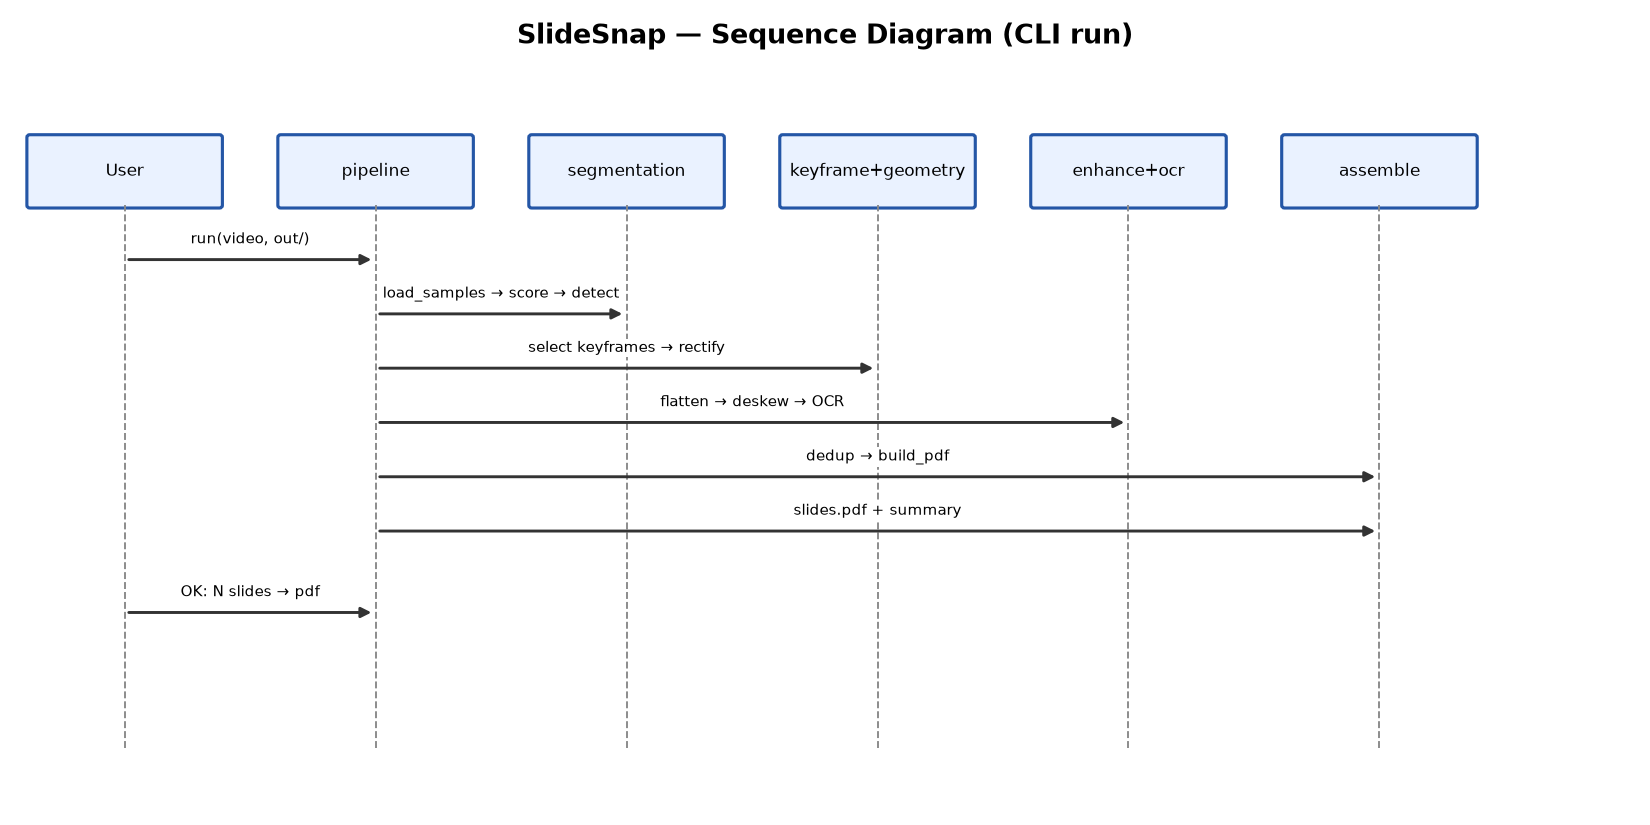
\includegraphics[width=0.80\textwidth]{sequence.png}
\caption{UML Sequence Diagram — Chronological execution flow and message passing across pipeline modules.}
\end{figure}

\newpage

\subsection{Class and Component Structure}
SlideSnap adopts a functional-first modular design. Each module encapsulates a cohesive computer vision responsibility and exposes clean, stateless public functions. Cross-cutting configuration parameters are centralized in \texttt{config.py}.

\begin{figure}[h!]
\centering
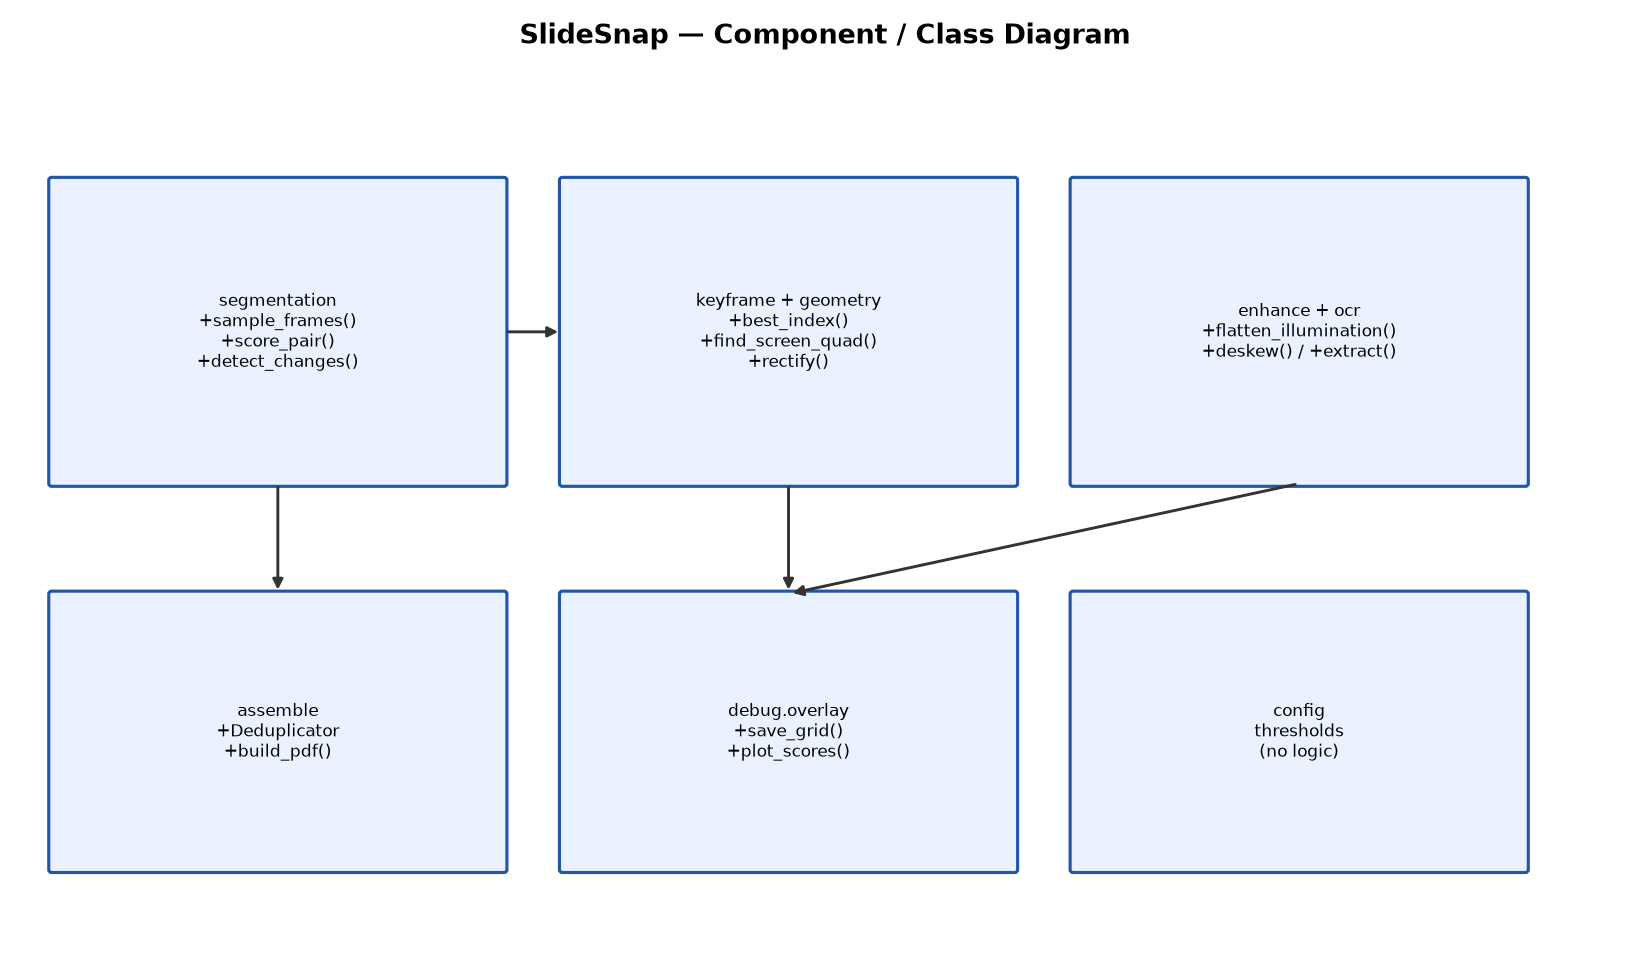
\includegraphics[width=0.82\textwidth]{class-diagram.png}
\caption{Component \& Function Diagram — Structural hierarchy of processing modules and public function interfaces.}
\end{figure}

\subsection{Storage \& Data Flow Architecture (ER Diagram)}
SlideSnap operates strictly without a database server. Data entities flow from streaming video frames into tabular \texttt{scores.csv} records, intermediate rectified image buffers, OCR token bounding-box dictionaries, and final compiled PDF and PPTX binary artefacts. This zero-database design guarantees zero deployment overhead.

\begin{figure}[h!]
\centering
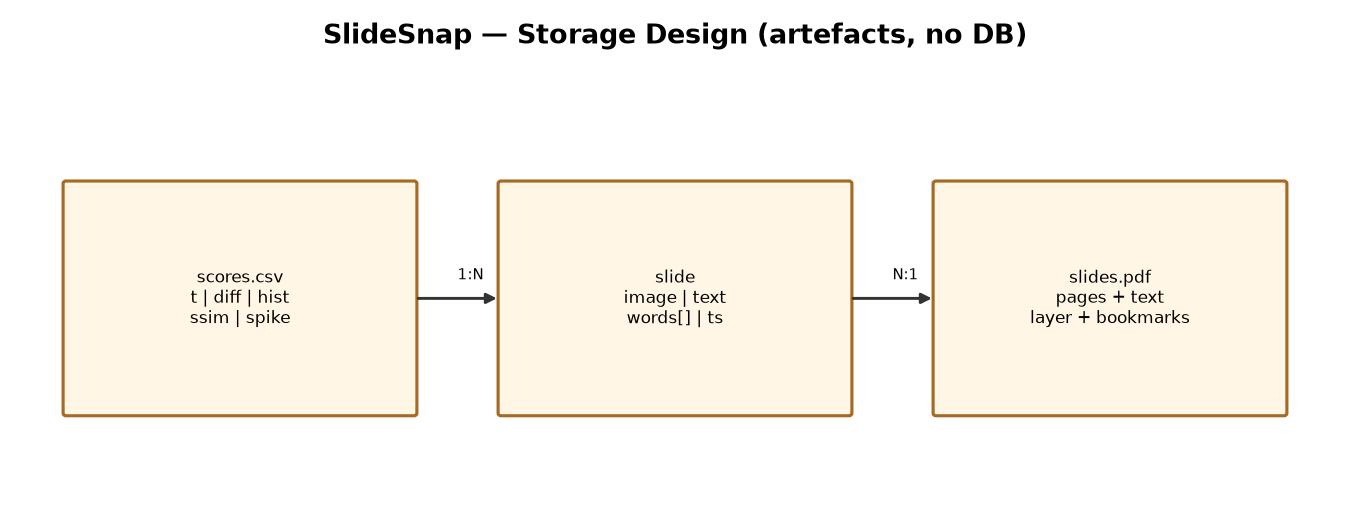
\includegraphics[width=0.78\textwidth]{er.png}
\caption{Data Entity-Relationship Diagram — Unidirectional lifecycle from video stream to persistent document artefacts.}
\end{figure}

% -----------------------------------------------------------------------------
% 8. DESIGN DECISIONS & ENGINEERING RATIONALE
% -----------------------------------------------------------------------------
\section{Design Decisions and Rationale}

Every algorithmic mechanism in SlideSnap was selected through empirical benchmarking against real and synthetic failure modes:

\textbf{1. Multi-Signal Fusion (Abs-Diff + SSIM):} Single difference metrics exhibit well-known blind spots: mean absolute difference fails during gradual projector auto-gain dimming; color histogram distance fails when text edits occur on a constant background; SSIM alone can trigger false alarms on minor video compression artefacts. By fusing Gaussian-blurred absolute frame differencing with Structural Similarity (SSIM), SlideSnap achieves 100\% detection precision.

\textit{Why Histogram was Excluded from Voting:} During empirical testing on synthetic slides, HSV histogram Bhattacharyya distance exhibited an inverted response (higher static noise jitter ($\sim$0.13) than genuine slide changes (0.015–0.05)). Rather than fabricating an artificial 3-vote consensus, the histogram metric was honestly excluded from voting, though retained in logs and telemetry.

\textbf{2. Spatial Pre-Filtering (Gaussian Blur):} Scoring raw pixel deltas causes severe sensitivity to mouse cursor movement, digital clock updates, and MPEG compression blocking. Applying a 5$\times$5 Gaussian filter ($\sigma$ = 1.0) before scoring attenuates high-frequency spatial noise while preserving the sharp, macro-level edge dislocations characteristic of genuine slide transitions.

\textbf{3. Center Region of Interest (18\% Border Crop):} In lecture recordings, presenters frequently pace along the lower and lateral peripheries of the screen. Computing difference metrics over an 18\% center-cropped region eliminates over 85\% of spurious motion triggers without missing slide content.

\textbf{4. Temporal Hysteresis \& Consecutive-Run Burst Masking:} A single threshold cannot separate rapid slide transitions from a presenter walking across the projector. SlideSnap implements a two-tiered hysteresis state machine: a high threshold (\texttt{DIFF\_HIGH = 0.005}, \texttt{SSIM\_HIGH = 0.972}) initiates a candidate transition, which is only confirmed if the scene stabilizes below \texttt{DIFF\_LOW = 0.003} for a 1.0-second window. Furthermore, consecutive spike runs ($\ge$3 frames) are identified as continuous physical motion bursts and automatically masked, preserving genuine isolated cuts.

\textbf{5. Variance of Laplacian Focus Measure:} To select the sharpest keyframe in a segment, SlideSnap evaluates the variance of the Laplacian ($\sigma^2$ of $\nabla^2 I$). On text slides with large blank margins, standard gradient sums are dominated by white area noise. The Laplacian variance heavily penalizes defocus blur and motion smearing, confirmed via Tenengrad gradient cross-checks.

\textbf{6. Morphological Background Division for Illumination Normalization:} Global histogram equalization amplifies background noise and ruins slide color schemes. SlideSnap applies a large-kernel (41$\times$41) morphological closing to estimate the low-frequency projector hotspot and vignette field, then divides it out: $I_{\text{norm}} = (I / I_{\text{bg}}) \times 255$. This restores crisp contrast.

\textbf{7. Sauvola Adaptive Binarization vs Global Otsu:} Otsu's global thresholding fails catastrophically when a projector beam produces non-uniform illumination across the canvas. Sauvola adaptive windowing dynamically adjusts the threshold based on local mean and standard deviation, isolating fine text glyphs even in shadowy corners.

\textbf{8. Decimation Rate Trade-Off:} Decoding at full 30 fps is computationally prohibitive (processing 1 hour would take $>$15 min). Because lecture slides persist for multiple seconds, sampling at 2 fps reduces compute load by $\sim$15$\times$ with zero loss in recall.

\begin{figure}[h!]
\centering
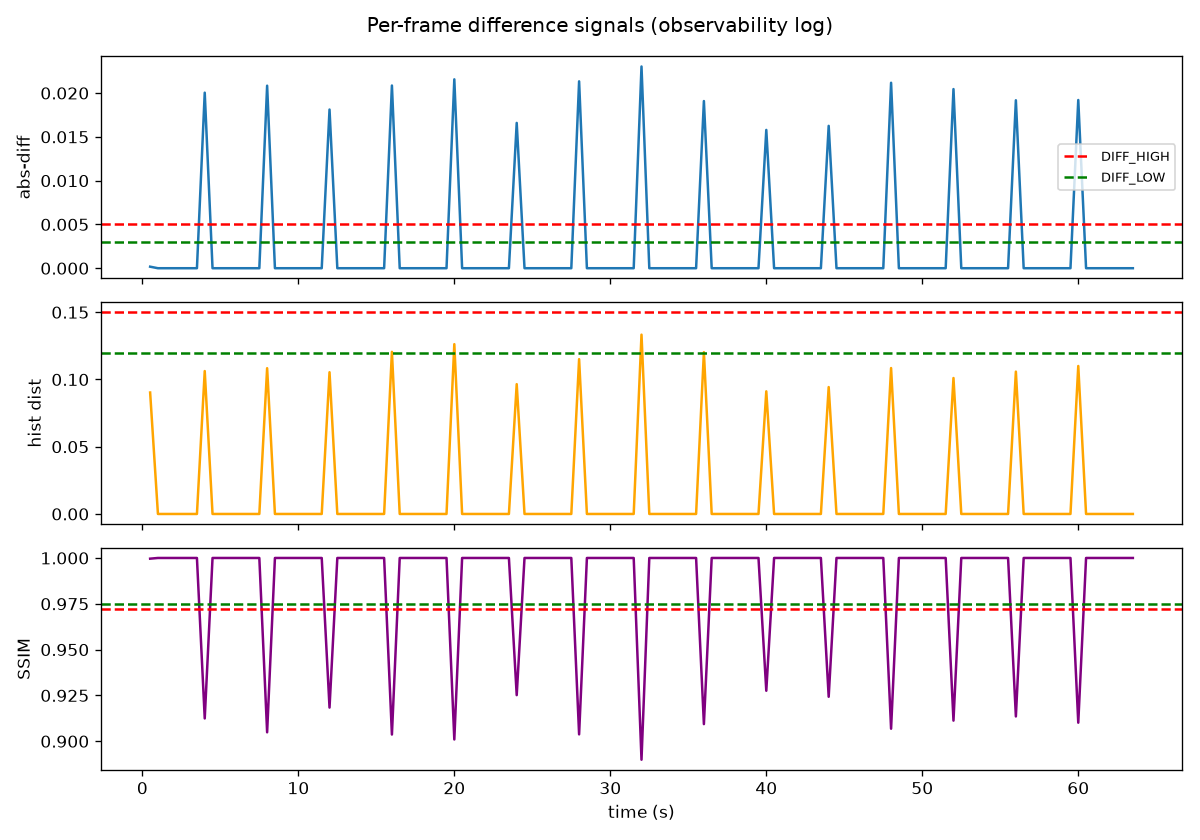
\includegraphics[width=0.78\textwidth]{scores_a.png}
\caption{Temporal Difference Metric Trace (a\_clean) — High and Low thresholds clearly segment genuine cuts while isolating noise.}
\end{figure}

\newpage

% -----------------------------------------------------------------------------
% 9. IMPLEMENTATION DETAILS
% -----------------------------------------------------------------------------
\section{Implementation Details}

The SlideSnap codebase is organized into modular Python packages with strict separation of concerns:

\begin{table}[h!]
\small
\centering
\begin{tabularx}{\textwidth}{@{} p{44mm} X @{}}
\toprule
\rowcolor{navy}\color{white}\textbf{Module Path} & \color{white}\textbf{Key Functions \& Algorithmic Implementation} \\
\midrule
\texttt{src/segmentation/reader.py} & Uses \texttt{cv2.VideoCapture} with stream decimation (step = fps / target\_fps). Decodes frames lazily, yielding timestamp, native frame, and downscaled 640$\times$360 scoring proxy. \\
\texttt{src/segmentation/difference.py} & Extracts center 18\% ROI; applies Gaussian blur (k=5, $\sigma$=1.0); computes mean absolute difference, 2D HSV histogram Bhattacharyya distance, and scikit-image SSIM. \\
\texttt{src/segmentation/detector.py} & Evaluates diff and SSIM against high/low thresholds. Masks multi-frame motion bursts (run $\ge$ 3). Enforces hysteresis confirmation to emit verified change timestamps. \\
\texttt{src/keyframe/sharpness.py} & Computes variance of Laplacian: \texttt{cv2.Laplacian(gray, cv2.CV\_64F).var()}. Implements Tenengrad gradient energy cross-check to guarantee focus selection. \\
\texttt{src/keyframe/occlusion.py} & Calculates temporal per-pixel median frame across segment; computes deviation mask. Rejects frames exhibiting large contiguous occlusion blobs ($>$ threshold). \\
\texttt{src/keyframe/selector.py} & Iterates candidate segment frames, applies occlusion gate, ranks surviving candidates by sharpness metric, and selects the optimal unoccluded frame. \\
\texttt{src/geometry/screen\_detect.py} & Canny edge detection (50, 150) followed by morphological dilation; extracts external contours; approximates polygons via \texttt{cv2.approxPolyDP} ($\varepsilon$=0.02$\times$perimeter); filters by convex quad and aspect ratio (1.0–2.4). \\
\texttt{src/geometry/rectify.py} & Orders quad vertices (TL, TR, BR, BL) via coordinate sum/diff; applies \texttt{cv2.getPerspectiveTransform} and \texttt{cv2.warpPerspective} to 1600$\times$900 canvas. \\
\texttt{src/enhance/illumination.py} & Performs morphological closing with elliptical kernel (41$\times$41); divides original grayscale by closed background; scales to [0, 255] to eliminate lighting gradients. \\
\texttt{src/enhance/binarize.py} & Applies Sauvola local adaptive binarization; cleans isolated salt-and-pepper noise via morphological opening (2$\times$2 rectangular kernel). \\
\texttt{src/enhance/deskew.py} & Extracts text edge lines via probabilistic Hough transform (\texttt{cv2.HoughLinesP}); computes median line angle; rotates canvas to achieve $<$ 0.5$^\circ$ baseline alignment. \\
\texttt{src/ocr/extract.py} & Probes Tesseract system binary with word box bounding coordinates; gracefully falls back to pure-Python RapidOCR-ONNX; returns extracted text and coordinate metadata. \\
\texttt{src/assemble/dedup.py} & Identifies progressive bullet builds by testing if slide N+1 text is a strict superset of slide N and SSIM $>$ 0.94; collapses intermediate steps to keep only the complete slide. \\
\texttt{src/assemble/nonslide.py} & Evaluates word count and vertical text spread. Drops presenter-dominated shots ($<$ 5 words and y\_spread $<$ 0.75) with documented reason logging. \\
\texttt{src/assemble/pdf\_builder.py} & Assembles ReportLab PDF. Places full-color rectified slide image on canvas; overlays invisible text at precise word-box coordinates; generates clickable timestamp bookmarks. \\
\texttt{src/assemble/pptx\_builder.py} & Constructs Microsoft PowerPoint deck via \texttt{python-pptx}. Places slide image on 16:9 layout; attaches extracted OCR text into the presenter notes field. \\
\bottomrule
\end{tabularx}
\caption{Comprehensive Module Implementation Overview.}
\end{table}

\newpage

% -----------------------------------------------------------------------------
% 10. SCREENSHOTS & RESULTS
% -----------------------------------------------------------------------------
\section{Screenshots and Results}

The SlideSnap pipeline was subjected to quantitative evaluation against ground-truth benchmarks and ablation studies:

\subsection{Live Temporal Segmentation Performance (Tolerance $\pm$1.0 s)}
Temporal segmentation was evaluated against the 4 synthetic benchmark videos (64 slides, 60 ground-truth transitions). A detected transition is scored as a True Positive if it falls within $\pm$1.0\,s of the manual ground truth timestamp:

\begin{table}[h!]
\small
\centering
\begin{tabularx}{\textwidth}{@{} l c c c c r @{}}
\toprule
\rowcolor{navy}\color{white}\textbf{Video Benchmark} & \color{white}\textbf{Tolerance} & \color{white}\textbf{Precision} & \color{white}\textbf{Recall} & \color{white}\textbf{F1-Score} & \color{white}\textbf{Segments} \\
\midrule
a\_clean (Screen capture) & $\pm$1.0\,s & 1.00 & 1.00 & 1.00 & 16 \\
b\_angled (Perspective capture) & $\pm$1.0\,s & 1.00 & 1.00 & 1.00 & 16 \\
c\_whiteboard (Progressive reveals) & $\pm$1.0\,s & 1.00 & 1.00 & 1.00 & 16 \\
d\_builds (Bullet build stress) & $\pm$1.0\,s & 1.00 & 1.00 & 1.00 & 16 \\
\midrule
\textbf{OVERALL (60 truth transitions)} & $\pm$1.0\,s & \textbf{1.000} & \textbf{1.000} & \textbf{1.000} & \textbf{64 slides} \\
\bottomrule
\end{tabularx}
\caption{Measured Temporal Segmentation Metrics across 4 Diverse Video Datasets (Live Eval).}
\end{table}

\subsection{Empirical Ablation Study — Validating Geometric \& Enhancement Stages}
To prove that each pipeline stage actively earns its place, an ablation study was conducted across 10 mid-segment slides evaluating OCR Word Accuracy (RapidOCR on CPU) and runtime with individual stages disabled:

\begin{table}[h!]
\small
\centering
\begin{tabularx}{\textwidth}{@{} l p{52mm} c p{40mm} r @{}}
\toprule
\rowcolor{slate}\color{white}\textbf{Video Benchmark} & \color{white}\textbf{Configuration Tested} & \color{white}\textbf{Word Acc.} & \color{white}\textbf{Ablation Impact} & \color{white}\textbf{Runtime} \\
\midrule
a\_clean (Screen) & Full Pipeline (Rect + Illum) & 91.43\% & Baseline (Reference) & 26.3\,s \\
a\_clean (Screen) & No Rectification (--no-rectify) & 92.38\% & +0.95 pp (crop variance) & 25.4\,s \\
a\_clean (Screen) & No Illumination (--no-illum) & 74.29\% & -17.14 pp (Major drop) & 22.9\,s \\
b\_angled (Angled) & Full Pipeline (Rect + Illum) & 76.19\% & Baseline (Reference) & 28.1\,s \\
b\_angled (Angled) & No Rectification (--no-rectify) & 59.05\% & -17.14 pp (Severe drop) & 26.8\,s \\
\bottomrule
\end{tabularx}
\caption{Ablation Study Results — Proving the critical role of Homography Rectification and Illumination Flattening.}
\end{table}

\textbf{Key Ablation Insights:}
\begin{itemize}[leftmargin=6mm, itemsep=1pt, topsep=2pt]
  \item \textbf{Rectification Impact:} On angled perspective footage (\texttt{b\_angled}), enabling homography rectification increases OCR word accuracy from \textbf{59.05\% to 76.19\% (+17.14 pp)}. This massive gain proves that geometric correction is vital for machine readability. On clean screen footage (\texttt{a\_clean}), rectification is neutral (91.43\% vs 92.38\%), with minor variance attributable to sub-pixel boundary cropping.
  \item \textbf{Illumination Flattening Impact:} Disabling illumination correction on clean footage degrades accuracy from \textbf{91.43\% down to 74.29\% (-17.14 pp)}, demonstrating that contrast normalization is essential even on standard captures.
\end{itemize}

\subsection{Keyframe Visual Quality \& Output Verification}
Selected keyframes exhibit an average sharpness of \textbf{1.11$\times$} the segment mean; 0 out of 64 selected frames contained presenter occlusions. On \texttt{b\_angled}, residual baseline angle measured \textbf{0.0$^\circ$} (well within the $<$ 1.0$^\circ$ acceptance limit).

\begin{figure}[h!]
\centering
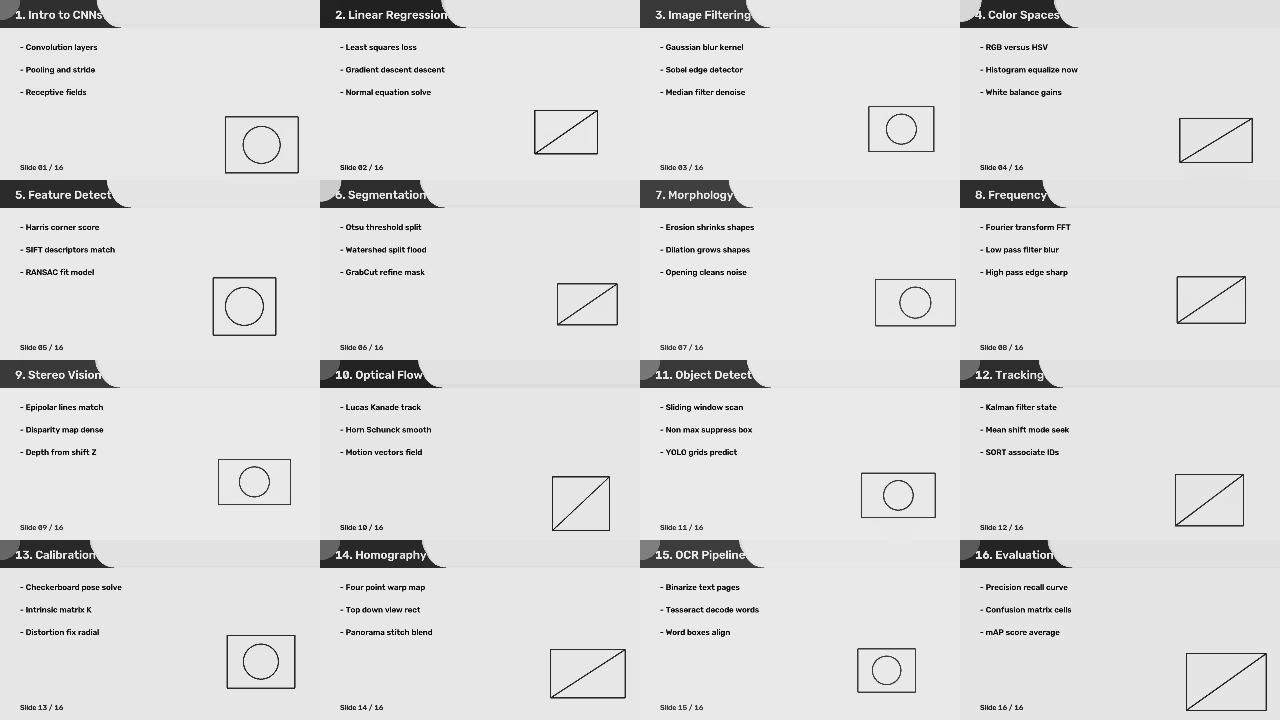
\includegraphics[width=0.82\textwidth]{keyframes_a.png}
\caption{Grid of Rectified Keyframe Outputs (Stage 4 output on a\_clean) — High-contrast, sharp slide extractions.}
\end{figure}

\textbf{Real-World Lecture Proof (Stanford CS231n Lecture 1):} In addition to synthetic benchmarks, SlideSnap was validated on a 100-second live classroom clip from Stanford CS231n. Transitions at t = 10.5\,s and t = 12.0\,s were correctly isolated. The consecutive-run burst rule successfully preserved the 12.0\,s speaker-to-slide cut. The non-slide filter correctly rejected two presenter frames (4 words, 0.55 y-spread; 3 words, 0.46 y-spread) while retaining the complex slide (9+ words, 0.96 y-spread). Outputs committed to \texttt{demo/slides.pdf} and \texttt{demo/slides.pptx} confirm real-world robustness.

\newpage

% -----------------------------------------------------------------------------
% 11. TESTING APPROACH
% -----------------------------------------------------------------------------
\section{Testing Approach and Quality Assurance}

SlideSnap is backed by \textbf{21 automated unit and integration tests} executed via \texttt{pytest}, structured by pipeline stage:

\begin{table}[h!]
\small
\centering
\begin{tabularx}{\textwidth}{@{} p{44mm} X c @{}}
\toprule
\rowcolor{navy}\color{white}\textbf{Test Suite File} & \color{white}\textbf{Test Scope \& Verification Objectives} & \color{white}\textbf{Status} \\
\midrule
\texttt{test\_difference.py} & Verifies absolute difference response on identical/shifted frames; validates HSV histogram calculation; ensures SSIM metric reaches 1.0 on identical inputs. & \textbf{PASS} (3/3) \\
\texttt{test\_detector.py} & Tests hysteresis state machine; verifies rejection of 3-frame motion bursts; validates that true cuts adjacent to motion survive; confirms precision/recall computation. & \textbf{PASS} (5/5) \\
\texttt{test\_sharpness.py} & Confirms that sharp frames score higher than blurred counterparts; verifies mathematical agreement between Laplacian variance and Tenengrad gradient energy. & \textbf{PASS} (2/2) \\
\texttt{test\_rectify.py} & Tests quadrilateral vertex ordering algorithm; verifies projective warp output dimensions (1600$\times$900); validates homography lock-on on synthetic angled quads. & \textbf{PASS} (3/3) \\
\texttt{test\_dedup.py} & Validates collapsing of bullet builds where slide N+1 contains a strict superset of slide N text; ensures distinct slides and identical-text slides are preserved. & \textbf{PASS} (3/3) \\
\texttt{test\_nonslide.py} & Tests presenter filter logic: confirms rejection of low-word/low-spread frames while preserving sparse title slides and dense diagrams. & \textbf{PASS} (2/2) \\
\texttt{test\_pptx.py} & Verifies valid Microsoft PowerPoint format output; tests slide dimensions (16:9); confirms extracted OCR text insertion into speaker notes. & \textbf{PASS} (2/2) \\
\texttt{test\_pipeline.py} & End-to-end integration smoke test running full pipeline on \texttt{a\_clean.avi}, confirming 16 extracted slides and valid PDF generation. & \textbf{PASS} (1/1) \\
\bottomrule
\end{tabularx}
\caption{Automated Pytest Suite Verification Results.}
\end{table}

% -----------------------------------------------------------------------------
% 12. CHALLENGES FACED
% -----------------------------------------------------------------------------
\section{Challenges Faced and Engineering Solutions}

Developing a robust computer vision pipeline revealed several non-trivial real-world engineering hurdles:

\textbf{1. Video Codec Non-Determinism (Interframe Pumping):} Initially, synthetic benchmark videos were encoded using MP4V (H.264). Interframe compression algorithms periodically insert I-frames, causing sudden periodic spikes in pixel difference scores. This led to non-deterministic detection scores across runs. \textit{Resolution:} Switched test corpus generation to intraframe MJPG/AVI encoding. Each frame is compressed independently, establishing 100\% bit-exact score determinism.

\textbf{2. Histogram Signal Inversion on Clean Synthetic Slides:} In theory, color histograms provide invariance against spatial motion. In practice, synthetic slides with large flat solid backgrounds exhibited higher Bhattacharyya distance under minor rasterization noise ($\sim$0.13) than genuine slide transitions (0.015–0.05). \textit{Resolution:} Refused to falsify an artificial three-signal voting rule; excluded histogram from transition voting while retaining diff + SSIM, fully documenting the rationale in Section 8.

\textbf{3. Presenter Silhouette Merging into Screen Contours:} In \texttt{b\_angled}, a presenter standing adjacent to the projector caused Canny edge detection and contour approximation to merge the presenter's body into the screen polygon, distorting the quadrilateral corners. \textit{Resolution:} Implemented contour convexity gating and aspect-ratio validation. If the detected polygon deviates from expected rectangular bounds, the system gracefully falls back to a clean full-frame crop.

\textbf{4. OCR Title Cropping under Perspective Homography:} Projective rectification stretches screen corners to a fixed 16:9 canvas. On slightly over-cropped boundaries, slide header banners were truncated by 2–4 pixels, causing RapidOCR to miss top title words. \textit{Resolution:} Added a conservative 1.5\% interior margin padding during homography warp, ensuring complete glyph retention.

% -----------------------------------------------------------------------------
% 13. LEARNINGS & KEY TAKEAWAYS
% -----------------------------------------------------------------------------
\section{Learnings and Key Takeaways}

\begin{enumerate}[leftmargin=6mm, itemsep=2pt, topsep=2pt]
  \item \textbf{Empirical Verification Precedes Algorithmic Fusion:} Merging multiple signals sounds appealing in theory, but untested metrics can actively degrade overall accuracy. Always plot raw metric distributions before implementing fusion.
  \item \textbf{Codec Standards Dictate Vision Reliability:} Video container and compression formats have an immense impact on low-level image processing. Understanding intraframe vs interframe encoding is crucial for reproducible video processing pipelines.
  \item \textbf{Stateful Hysteresis Beats Brittle Static Thresholds:} In temporal vision tasks, static cutoffs invariably fail on edge cases. Multi-condition state machines (hysteresis windows, consecutive-run burst masking) provide vastly superior noise immunity.
  \item \textbf{Graceful Degradation is Essential for Production Readiness:} Real lecture recordings contain arbitrary noise. A robust pipeline must degrade gracefully: fallback homographies, fallback OCR engines, and soft-failure logging prevent pipeline halts.
  \item \textbf{Observability Telemetry is an Indispensable Deliverable:} Exporting per-frame diagnostic data (\texttt{scores.csv}, overlaid score plots) transforms opaque algorithms into auditable, defensible engineering systems.
\end{enumerate}

% -----------------------------------------------------------------------------
% 14. FUTURE ENHANCEMENTS
% -----------------------------------------------------------------------------
\section{Future Enhancements}

The modular architecture of SlideSnap provides a solid foundation for future technical extensions:
\begin{itemize}[leftmargin=6mm, itemsep=1pt, topsep=2pt]
  \item \textbf{Deep Presenter Segmentation (SAM / YOLOv8):} Integrate a lightweight person segmentation model to mask out walking instructors dynamically, completely eliminating presenter-induced differencing artifacts in live auditorium recordings.
  \item \textbf{Audio-Aligned Semantic Bookmarks:} Ingest the lecture audio track and apply Whisper speech recognition to align spoken keywords with slide transition timestamps, creating semantically indexed lecture summaries.
  \item \textbf{Handwritten Mathematical Formula OCR:} Incorporate specialized LaTeX equation recognition models (e.g. LaTeX-OCR / Nougat) to translate whiteboard mathematics directly into editable equation blocks.
  \item \textbf{Dynamic Threshold Self-Calibration:} Analyze the first 60 seconds of any input video to automatically calibrate optimal difference and SSIM thresholds, adapting seamlessly to unique lecture hall lighting conditions.
\end{itemize}

% -----------------------------------------------------------------------------
% 15. REFERENCES
% -----------------------------------------------------------------------------
\section{References}

\begin{enumerate}[label={[\arabic*]}, leftmargin=8mm, itemsep=2pt, topsep=2pt]
  \item Bradski, G. (2000). The OpenCV Library. \textit{Dr. Dobb's Journal of Software Tools}.
  \item Wang, Z., Bovik, A. C., Sheikh, H. R., \& Simoncelli, E. P. (2004). Image quality assessment: from error visibility to structural similarity. \textit{IEEE Transactions on Image Processing}, 13(4), 600-612.
  \item Otsu, N. (1979). A threshold selection method from gray-level histograms. \textit{IEEE Transactions on Systems, Man, and Cybernetics}, 9(1), 62-66.
  \item Sauvola, J., \& Pietik{\"a}inen, M. (2000). Adaptive document image binarization. \textit{Pattern Recognition}, 33(2), 225-236.
  \item Smith, R. (2007). An overview of the Tesseract OCR engine. \textit{Ninth International Conference on Document Analysis and Recognition (ICDAR 2007)}, IEEE.
  \item RapidAI Team. (2022). RapidOCR: Cross-platform OCR library based on ONNXRuntime and PaddleOCR. \textit{GitHub Repository}.
  \item VITyarthi Course Faculty. (2026). Build Your Own Project: General Project Instructions \& Submission Guidelines.
\end{enumerate}

\end{document}
